\documentclass[12pt]{article}
\usepackage{graphicx,amsmath}

\oddsidemargin  -0.5 cm
\evensidemargin 0.0 cm
\textwidth      6.5in
\headheight     0.0in
\topmargin      -1 cm
\textheight=9in

\renewcommand{\arraystretch}{1.25}

\title{Measuring Track Resolution from $K_S \to \pi^+\pi^-$}
\author{Jim Pivarski}

\begin{document}
\maketitle

\section{Motivation}

Optimizing the resolution of tracking detectors is only the first step
in searches for new phenomena; once the resolution has been improved
as much as possible, it must then be precisely known.  The
significance of new multi-track resonances is inversely proportional
to the resolution of such peaks: if observed, the resolution of the
peak can be derived from the observation, but if not, it will need to
be estimated to set the correct upper limit.  The easiest way to
estimate the resolution is from a Monte Carlo simulation, but in the
early stages of an experiment, the simulation might be missing
important effects.  One would be much more confident in the simulation
if it is confirmed by an independent measurement.

In simple cases, such as searches for new dimuon resonances, one could
imagine extrapolating from the widths of known peaks, $J/\psi$,
$\Upsilon$, and $Z$, without neededing to know the resolution of the
individual tracks.  However, new particles by definition have
unfamiliar kinematics: either the mass is much higher than any known
resonance or the momentum is, as new low-mass dimuons would have to be
produced from heavy top-down decays, necessarily giving them a much
higher boost than the $J/\psi$ or $\Upsilon$ mesons produced by strong
interactions.  Dimuon extrapolations would not be valid, because
boosted low-mass resolution depends on the underlying tracks'
curvature and initial directions in a different way from unboosted
low-mass resolution.

To derive the resolution of any prompt multi-track decay, it is
sufficient to know the track 3-momentum resolution as a probability
distribution, that is
\begin{equation}
P(\Delta q/p_T, \Delta \phi, \Delta \cot\theta; p_T, \phi, \eta, d_{xy}, d_z)
\label{eqn:resolution}
\end{equation}
where $\Delta q/p_T$, $\Delta \phi$, and $\Delta \cot\theta$ are the
differences between measured curvature, azimuthal angle, and cotangent
of the polar angle ($\cot\theta = p_z/p_T$) and their true values,
such that
\begin{equation}
\int d(\Delta q/p_T) \, d(\Delta \phi) \, d(\Delta \cot\theta) \,
P(\Delta q/p_T, \Delta \phi, \Delta \cot\theta; q p_T, \phi, \eta, d_{xy}, d_z) =
1\mbox{.}
\end{equation}
The arguments after the semicolon, $q p_T$, $\phi$, $\eta$, $d_{xy}$
and $d_z$, characterize the tracks in terms of their signed transverse
momentum, azimuthal angle, pseudorapidity, and transverse and
longitudinal impact parameters.  The above distribution can be
parameterized or expressed in bins of the most important arguments,
usually $q p_T$, $\eta$, and $d_{xy}$.

We can obtain the resolution distribution from Monte Carlo by
subtracting generator-level values from the reconstructed values of
each momentum component.  However, if it can also be derived directly
from the data, then we can perform an important check on the Monte
Carlo and also replace it in kinematic simulations, if the data-driven
distribution is known with sufficient precision.

\subsection{Split cosmic rays}

One way to derive the distribution in Equation~\ref{eqn:resolution} is
to acquire a sample of cosmic rays traversing the detector close to
the interaction point.  By reconstructing the two halves of the cosmic
ray's trajectory as separate tracks, we obtain independent
measurements of not only the three momentum components, but also the
two impact parameters; in other words,
\begin{equation}
P_{\mbox{\scriptsize cosmic}}(\Delta q/p_T, \Delta \phi, \Delta
\cot\theta, \Delta d_{xy}, \Delta d_z; q p_T, \phi, \eta, d_{xy},
d_z)\mbox{.}
\end{equation}
If one of the two tracks could be perfectly measured, then the
resolution of the other one would be derived by simply subtracting
each of the five parameters, track by track.  This would yield the
full 5-D distribution $P_{\mbox{\scriptsize cosmic}}$, with all the
correlations between the parameters intact.  Neither track can be
perfectly measured, but we can assume that they have the same
resolution and derive the final distribution by deconvolution.  For
Gaussian distributions centered on zero, convolution simply adds
widths in quadrature, so the single track resolution is approximately
\begin{equation}
\left(\begin{array}{l}
\Delta q/p_T \\
\Delta \phi \\
\Delta \cot\theta \\
\Delta d_{xy} \\
\Delta d_z \\
\end{array}\right) = \frac{1}{\sqrt{2}}
\left(\begin{array}{c}
(q/p_T)_1 - (q/p_T)_2 \\
\phi_1 - \phi_2 \\
\cot\theta_1 - \cot\theta_2 \\
(d_{xy})_1 - (d_{xy})_2 \\
(d_z)_1 - (d_z)_2 \\
\end{array}\right)\mbox{.}
\end{equation}

Though it is useful to have such a simple method to measure all five
track parameters, cosmic rays do have some disadvantages:
\begin{itemize}
\item Their distribution is primarily vertical, illuminating the top
  and bottom of the detector well, but not the sides or endcaps.  To
  extend the measurement to the sides of the detector, we can assume
  symmetry in $\phi$.  But it would be meaningless to extrapolate a
  barrel measurement (low $\eta$) to the endcaps (high $\eta$), where
  a different geometry and a different detector technology is used.
\item Only a small fraction pass close enough to the interaction point
  to resemble the tracks from collision products, whose resolution we
  want to determine.  One must either apply a tight cut on $d_{xy}$
  and $d_z$ or compute a $d_{xy} \to 0$, $d_z \to 0$ limit, which is
  essentially the same thing.
\item The pair of tracks under comparison always includes one top
  track and one bottom track, so it cannot resolve symmetric errors.
\item The top track traverses the detector in the ``wrong'' direction,
  opposite to tracks from collisions.  While this has several
  consequences, the most important is that cones from any associated
  showers, such as from TeV muons, point toward the interaction point
  instead of away from it.  This could make the resolution of the top
  track different from that of the bottom track.
\item The number of collected cosmic rays does not scale with
  luminosity, so the statistical gain diminishes with time.
\end{itemize}

The two advantages which are unique to this cosmic ray technique are:
(1) access to all five track parameters, and (2) the cosmic ray
spectrum is power-law, rather than exponential, so it can supply
higher-energy events than any other technique.

\subsection{Dimuon resonance masses}

The $J/\psi$ and $\Upsilon$ families and the $Z$ boson decay into muon
pairs with known masses, providing an a priori constraint for each
event.  Unfortunately, one constraint is not enough to fully analyze
the tracks: the other parameters would need to be presumed to be
correctly measured or deconvolved from an assumed resolution.

For example, in $Z\to\mu^+\mu^-$ decays, the $Z$ boson has an unknown
3-momentum, though its vertex can be assumed to coincide with the
nearest primary vertex (constructed using all tracks except the two
muons).  To compute $\Delta q/pT$ of the first track, we must use all
the measured track parameters of the second track, as well as $\phi$
and $\cot\theta$ of the first track.  To account for the uncertainty
in these five reference parameters, as well as the intrinsic width of
the $Z$, one can deconvolve the final distribution using a technique
described later in this note.  Applying this method would improve our
knowledge of curvature $q/pT$, but not $\Delta \phi$ or $\Delta
\cot\theta$.

For tracks with high enough momenta to be regarded as being
essentially straight, such as high-energy $Z$ daughters, the
momentum resolution is dominated by the second-order curvature
measurement, rather than first-order $\Delta \phi$ or $\Delta
\cot\theta$.  However, for lower momenta, $\Delta q/pT$ and $\Delta
\phi$ are more tightly coupled, so a different technique would be
needed.

\section{Kinematic constraints from $K_S \to \pi^+\pi^-$}

Two-body decays of $K_S$ differ from the dimuon resonances considered
above in that $K_S$ has a macroscopic flight path of several
centimeters--- long enough to accurately measure its direction but
short enough to resemble the prompt tracks of interest.  A diagram of
the event topology is given in Figure~\ref{fig:diagram}.

\begin{figure}
\begin{center}
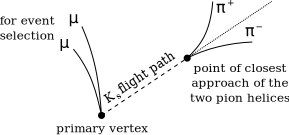
\includegraphics[width=0.65\linewidth]{diagram.pdf}
\end{center}
\caption{Schematic diagram of $K_S \to \pi^+\pi^-$ from a hadron collision. \label{fig:diagram}}
\end{figure}

The direction of the $K_S$ momentum ($\phi_K$, $\theta_K$) can be
determined from the displacement vector between the primary vertex and
the $\pi^+\pi^-$ vertex (defined by their point of closest approach).
Though the magnitude of that displacement is random, its direction
must coincide with the $K_S$ momentum.  These two constraints combine
with the known $K_S$ mass to completely determine its kinematics.

To demonstrate the usefulness of this topology, we can show that the
3-momentum $\vec{p}_+$ of one daughter $\pi^+$ can be completely
determined from the 3-momentum $\vec{p}_-$ of the other and the
displacement vector $\vec{s}$ between the two vertices.  The $K_S$
3-momentum is the sum of $\vec{p}_+$ and $\vec{p}_-$, and also
$\vec{s}$ scaled by a factor $\alpha$:
\begin{equation}
\vec{p}_+ + \vec{p}_- = \alpha \vec{s}\mbox{.}
\end{equation}
The mass constraint determines $\alpha$:
\begin{eqnarray}
\left(\sqrt{|\vec{p}_+|^2 + {m_\pi}^2} + \sqrt{|\vec{p}_-|^2 + {m_\pi}^2}\right)^2 - \left(\vec{p}_+ + \vec{p}_-\right)^2 = {m_{K_S}}^2 \\
\left(\sqrt{|\alpha \vec{s} - \vec{p}_-|^2 + {m_\pi}^2} + \sqrt{|\vec{p}_-|^2 + {m_\pi}^2}\right)^2 - \alpha^2 |\vec{s}|^2 = {m_{K_S}}^2\mbox{.}
\end{eqnarray}
Expand and collect terms, with many cancellations:
\begin{multline}
\alpha^2 \bigg(|\vec{s}|^2\left(|\vec{p}_-|^2 + {m_\pi}^2\right) - \left(\vec{s} \cdot \vec{p}_-\right)^2\bigg)
+ \alpha \bigg(-{m_{K_S}}^2 \left(\vec{s} \cdot \vec{p}_-\right) \bigg) \\
+ \left({m_{K_S}}^2 \left(|\vec{p}_-|^2 + {m_\pi}^2\right) - \frac{{m_{K_S}}^4}{4}\right) = 0
\end{multline}
\begin{equation}
\alpha = \frac{{m_{K_S}}^2 \left(\vec{s} \cdot \vec{p}_-\right) \pm 2 m_{K_S} \sqrt{\left(|\vec{p}_-|^2 + {m_\pi}^2\right)
\left[\left(\vec{s} \cdot \vec{p}_-\right)^2 - |\vec{s}|^2 \left(|\vec{p}_-|^2 + {m_\pi}^2 - \frac{{m_{K_S}}^2}{4} \right)\right]}}
{2 \bigg(|\vec{s}|^2 \left(|\vec{p}_-|^2 + {m_\pi}^2\right) - \left(\vec{s} \cdot \vec{p}_-\right)^2\bigg)}\mbox{.}
%% \alpha = \frac{{m_{K_S}}^2 \left(\vec{s} \cdot \vec{p}_-\right) \pm \sqrt{{m_{K_S}}^4 \left(\vec{s} \cdot \vec{p}_-\right)^2
%% - 4 \bigg(|\vec{s}|^2 \left(|\vec{p}_-|^2 + {m_\pi}^2\right) - \left(\vec{s} \cdot \vec{p}_-\right)^2\bigg)
%% \bigg({m_{K_S}}^2 \left(|\vec{p}_-|^2 + {m_\pi}^2\right) - \frac{{m_{K_S}}^4}{4}\bigg)}}{2 |\vec{s}|^2 \bigg(\left(|\vec{p}_-|^2 + {m_\pi}^2\right) - \left(\vec{s} \cdot \vec{p}_-\right)^2\bigg)}\mbox{.}
\end{equation}
And thus we can cross-check each component of $\vec{p}_+$ with data
derived from $\vec{p}_-$ and the $\pi^+\pi^-$ vertex, with only a twofold
degeneracy in solutions ($\pm$ in the solution for $\alpha$).
\begin{equation}
\left(\begin{array}{c}
\Delta {p_x}_+ \\
\Delta {p_y}_+ \\
\Delta {p_z}_+ \\
\end{array}\right) \mbox{ should be equal to }
\left(\begin{array}{c}
\alpha s_x - {p_x}_- \\
\alpha s_y - {p_y}_- \\
\alpha s_z - {p_z}_- \\
\end{array}\right)
\label{eqn:pplus_in_terms_of_pminus}
\end{equation}

The right-hand side of Equation~\ref{eqn:pplus_in_terms_of_pminus}
contains a hidden dependency on the $\pi^+$ track, in that the
$\pi^+\pi^-$ vertex, and therefore $\vec{s}$, cannot be determined
without knowing all of the $\pi^+$ track parameters.  However, that
calculation depends crucially on the $\pi^+$ impact parameters, so the
test is not trivially satisfied.

\section{Deriving track resolution from constraints}

More generically, we can say that we observe four constraints in the
$K_S\to\pi^+\pi^-$ decay which are a function $f$ of the measured
track parameters of the pions (randomly labeled track~1 and
track~2)
\begin{equation}
\left(\begin{array}{c}
\left.m_{K_S}\right|_{\mbox{\scriptsize true}} - \left.m_{K_S}\right|_{\mbox{\scriptsize tracks}} \\
\left.\phi_{K_S}\right|_{\mbox{\scriptsize vertex}} - \left.\phi_{K_S}\right|_{\mbox{\scriptsize tracks}} \\
\left.\cot\theta_{K_S}\right|_{\mbox{\scriptsize vertex}} - \left.\cot\theta_{K_S}\right|_{\mbox{\scriptsize tracks}} \\
\left.z\right|_{\pi^+} - \left.z\right|_{\pi^-} \\
\end{array}\right) =
f\left(\begin{array}{r}
\left.q/p_T\right|_1 \\
\left.\phi\right|_1 \\
\left.\cot\theta\right|_1 \\
\left.d_z\right|_1 \\
\left.d_{xy}\right|_1 \\
\left.q/p_T\right|_2 \\
\left.\phi\right|_2 \\
\left.\cot\theta\right|_2 \\
\left.d_z\right|_2 \\
\left.d_{xy}\right|_2 \\
\end{array}\right)
\end{equation}
where the first three terms on the left-hand-side are a rearrangement
of the momentum constraint we discussed in the previous section, and
$\left.z\right|_{\pi^+} - \left.z\right|_{\pi^-}$ is an additional
constraint on the impact parameters: the distance of closest approach
of the two helices gives us information about the tracks' $d_{xy}$ and
$d_z$ because that distance ought to be zero.  We can only measure
one, and we choose $d_z$ because it will be more significant after
deconvolving the effect of $d_{xy}$ than the reverse.

We are interested in the small region where the left-hand-side is
nearly zero, where we can expand the right-hand-side linearly around
the true values of the parameters.  (The left-hand-side is exactly
zero when the measured values are equal to the true values.)
\begin{equation}
\left(\begin{array}{c}
\left.m_{K_S}\right|_{\mbox{\scriptsize true}} - \left.m_{K_S}\right|_{\mbox{\scriptsize tracks}} \\
\left.\phi_{K_S}\right|_{\mbox{\scriptsize vertex}} - \left.\phi_{K_S}\right|_{\mbox{\scriptsize tracks}} \\
\left.\cot\theta_{K_S}\right|_{\mbox{\scriptsize vertex}} - \left.\cot\theta_{K_S}\right|_{\mbox{\scriptsize tracks}} \\
\left.z\right|_{\pi^+} - \left.z\right|_{\pi^-} \\
\end{array}\right) =
\left(\frac{\partial f_i}{\partial q_j}\right)
\left(\begin{array}{r}
\left.\Delta q/p_T\right|_1 \\
\left.\Delta \phi\right|_1 \\
\left.\Delta \cot\theta\right|_1 \\
\left.\Delta d_z\right|_1 \\
\left.\Delta d_{xy}\right|_1 \\
\left.\Delta q/p_T\right|_2 \\
\left.\Delta \phi\right|_2 \\
\left.\Delta \cot\theta\right|_2 \\
\left.\Delta d_z\right|_2 \\
\left.\Delta d_{xy}\right|_2 \\
\end{array}\right)
\label{eqn:tangent_space}
\end{equation}
The 4$\times$10 Jacobian matrix of the four $f_i$ components is
represented above as $\left(\frac{\partial f_i}{\partial q_j}\right)$.
We would like to derive the above errors in track parameters from the
constraints on the left, but the Jacobian cannot be inverted--- we can
only determine 4 of the 10 track parameters.  To select the first
four, we split the matrix into a 4$\times$4 part that we can invert
and a 4$\times$6 part corresponding to parameters whose uncertainty
will need to be deconvolved from the final result.

To split the matrix, we make two copies of it and mask alternate
blocks with zeros:
\begin{multline}
\left(\frac{\partial f_i}{\partial q_j}\right) =
\left(\begin{array}{c c c c c c c c c c}
f_{11} & f_{12} & f_{13} & f_{14} & 0 & 0 & 0 & 0 & 0 & 0 \\
f_{21} & f_{22} & f_{23} & f_{24} & 0 & 0 & 0 & 0 & 0 & 0 \\
f_{31} & f_{32} & f_{33} & f_{34} & 0 & 0 & 0 & 0 & 0 & 0 \\
f_{41} & f_{42} & f_{43} & f_{44} & 0 & 0 & 0 & 0 & 0 & 0 \\
\end{array}\right) + \\
\left(\begin{array}{c c c c c c c c c c}
0 & 0 & 0 & 0 & f_{15} & f_{16} & f_{17} & f_{18} & f_{19} & f_{10} \\
0 & 0 & 0 & 0 & f_{25} & f_{26} & f_{27} & f_{28} & f_{29} & f_{20} \\
0 & 0 & 0 & 0 & f_{35} & f_{36} & f_{37} & f_{38} & f_{39} & f_{30} \\
0 & 0 & 0 & 0 & f_{45} & f_{46} & f_{47} & f_{48} & f_{49} & f_{40} \\
\end{array}\right)
\end{multline}
\begin{equation}
\left(\partial f_{4\times 4}\right) = \left(\begin{array}{c c c c}
f_{11} & f_{12} & f_{13} & f_{14} \\
f_{21} & f_{22} & f_{23} & f_{24} \\
f_{31} & f_{32} & f_{33} & f_{34} \\
f_{41} & f_{42} & f_{43} & f_{44} \\
\end{array}\right) \mbox{ and }
\left(\partial f_{4\times 4}\right) = \left(\begin{array}{c c c c c c}
f_{15} & f_{16} & f_{17} & f_{18} & f_{19} & f_{10} \\
f_{25} & f_{26} & f_{27} & f_{28} & f_{29} & f_{20} \\
f_{35} & f_{36} & f_{37} & f_{38} & f_{39} & f_{30} \\
f_{45} & f_{46} & f_{47} & f_{48} & f_{49} & f_{40} \\
\end{array}\right)
\vspace{0.25 cm}
\end{equation}
which splits Equation~\ref{eqn:tangent_space} into
\begin{equation}
\left(\begin{array}{c}
\left.m_{K_S}\right|_{\mbox{\scriptsize true}} - \left.m_{K_S}\right|_{\mbox{\scriptsize tracks}} \\
\left.\phi_{K_S}\right|_{\mbox{\scriptsize vertex}} - \left.\phi_{K_S}\right|_{\mbox{\scriptsize tracks}} \\
\left.\cot\theta_{K_S}\right|_{\mbox{\scriptsize vertex}} - \left.\cot\theta_{K_S}\right|_{\mbox{\scriptsize tracks}} \\
\left.z\right|_{\pi^+} - \left.z\right|_{\pi^-} \\
\end{array}\right) =
\left(\partial f_{4\times 4}\right)
\left(\begin{array}{r}
\left.\Delta q/p_T\right|_1 \\
\left.\Delta \phi\right|_1 \\
\left.\Delta \cot\theta\right|_1 \\
\left.\Delta d_z\right|_1 \\
\end{array}\right) +
\left(\partial f_{4\times 6}\right)
\left(\begin{array}{r}
\left.\Delta d_{xy}\right|_1 \\
\left.\Delta q/p_T\right|_2 \\
\left.\Delta \phi\right|_2 \\
\left.\Delta \cot\theta\right|_2 \\
\left.\Delta d_z\right|_2 \\
\left.\Delta d_{xy}\right|_2 \\
\end{array}\right)\mbox{.}
\end{equation}
With a little rearrangement,
\begin{equation}
\left(\partial f_{4\times 4}\right)^{-1}
\left(\begin{array}{c}
\left.m_{K_S}\right|_{\mbox{\scriptsize true}} - \left.m_{K_S}\right|_{\mbox{\scriptsize tracks}} \\
\left.\phi_{K_S}\right|_{\mbox{\scriptsize vertex}} - \left.\phi_{K_S}\right|_{\mbox{\scriptsize tracks}} \\
\left.\cot\theta_{K_S}\right|_{\mbox{\scriptsize vertex}} - \left.\cot\theta_{K_S}\right|_{\mbox{\scriptsize tracks}} \\
\left.z\right|_{\pi^+} - \left.z\right|_{\pi^-} \\
\end{array}\right) =
\left(\begin{array}{r}
\left.\Delta q/p_T\right|_1 \\
\left.\Delta \phi\right|_1 \\
\left.\Delta \cot\theta\right|_1 \\
\left.\Delta d_z\right|_1 \\
\end{array}\right) + 
\left(\partial f_{4\times 4}\right)^{-1}
\left(\partial f_{4\times 6}\right)
\left(\begin{array}{r}
\left.\Delta d_{xy}\right|_1 \\
\left.\Delta q/p_T\right|_2 \\
\left.\Delta \phi\right|_2 \\
\left.\Delta \cot\theta\right|_2 \\
\left.\Delta d_z\right|_2 \\
\left.\Delta d_{xy}\right|_2 \\
\end{array}\right)\mbox{.}
\label{eqn:twoterms}
\end{equation}

The right-hand-side is the sum of deviates from two distributions, the
first is the distribution that we want, and the second is a
distribution that we can assume from a reasonable prior (the output of
a Monte Carlo simulation), transformed by matrices derived purely from
geometry.  The distribution of a sum of deviates from two
distributions is their convolution, so we will compute the desired
result by deconvolution.  The left-hand-side is the error distribution
measured in data, also transformed by a purely geometric matrix.  This
matrix would be difficult but possible to compute analytically, so a
calculation from numerical derivatives would be well-behaved.  To
derive the desired distribution, we will apply the transformations to
each measurement separately on the left-hand-side and each
randomly-generated deviate in the second term of the right-hand-side,
and then deconvolve the distribution of the latter from the
distribution of the former.

Although it was necessary to assume a distribution for the track~2
parameters and one of the impact parameters from track~1, the labels 1
and 2 were randomly assigned: the track~2 parameters must be
distributed in the same way as the track~1 parameters (in the same
$p_T$, $\eta$, and $d_{xy}$ bins).  This procedure improves our
knowledge of track~1 parameters with data: it can be repeated with the
assumed input being the result from iteration~1.  The only missing
piece is one of the two impact parameters, $\Delta d_{xy}$ in the
derivation above.  Applying this procedure will not improve our
knowledge of $\Delta d_{xy}$ (perhaps a 3-body decay would be
necessary).

\section{Deconvolving distributions}

Deconvolution of of parameterized distributions is much less
susceptible to numerical error than raw distributions in histograms,
so we begin by fitting distributions of the two terms in
Equation~\ref{eqn:twoterms} with the following ansatz:
\begin{equation}
g(\vec{x}) = \int d\vec{y} \, \left(\prod_i \frac{1}{\pi}\frac{\Gamma_i/2}{(x_i - y_i)^2 + (\Gamma_i/2)^2}\right)
\, \left(\prod_i \frac{1}{\sqrt{2\pi} \sigma_i} \right)\exp\left(\sum_i \frac{(x_i - a_i - \sum_{j>i} b_{ij} x_j)^2}{2 \, {\sigma_i}^2} \right)
\label{eqn:ansatz}
\end{equation}
The function is a convolution of a Cauchy-Lorentz distribution and a
Gaussian distribution for each parameter, with correlations $b_{ij}$ between
the Gaussians (to allow the error ellipse to be angled in the $i$, $j$
plane).  This is a highly descriptive function, with the Lorentz
$\Gamma_i$ absorbing any non-linear tails.  If there is non-negligible
background after applying the cuts described in the next section, we
should also include a constant or linear term to parameterize the
background, but not include it in the deconvolution.

When all functions are Fourier-transformed, convolution is simply
pointwise multiplication, so the easiest way to proceed is to
Fourier-transform each of the factors in Equation~\ref{eqn:ansatz}.
For the sake of this short note, we will operate on a simplified
ansatz:
\begin{equation}
g'(\vec{x}) = \int d\vec{y} \, \left(\prod_i \frac{1}{\pi}\frac{\Gamma_i/2}{(x_i - y_i)^2 + (\Gamma_i/2)^2}\right)
\, \left(\prod_i \frac{1}{\sqrt{2\pi} \sigma_i} \right)\exp\left(\sum_i \frac{(x_i - a_i)^2}{2 \, {\sigma_i}^2} \right)
\label{eqn:ansatz2}
\end{equation}
which reduces the complexity of the algebra (which would otherwise
involve a lot of polynomial fractions).  The Fourier transform of the
Cauchy-Lorentz distribution is
\begin{equation}
\frac{1}{\pi}\frac{\Gamma_i/2}{{x_i}^2 + (\Gamma_i/2)^2} \to \frac{1}{\sqrt{2\pi}} \exp\left(\frac{\Gamma_i}{2} |k_i|\right)\mbox{,}
\end{equation}
and the transform of the Gaussian is
\begin{equation}
\frac{1}{\sqrt{2\pi} \sigma_i} \exp\left(\frac{-(x_i - a_i)^2}{2 {\sigma_i}^2}\right) \to
\frac{1}{\sqrt{2\pi}} \exp\left(\frac{-{k_i}^2 {\sigma_i}^2}{2}\right) \exp(ia_i k_i)
\end{equation}
The Fourier transformation of our ansatz $g'(\vec{x})$ is simply the product of
these:
\begin{equation}
\hat{g}'(\vec{k}) = \prod_i \frac{1}{\sqrt{2\pi}} \exp\left(\frac{\Gamma_i}{2} |k_i|\right) \, \frac{1}{\sqrt{2\pi}} \exp\left(\frac{-{k_i}^2 {\sigma_i}^2}{2}\right) \exp(ia_i k_i)
\end{equation}
and the convolution of two such distributions with different
parameters, $g^A(\vec{x})$ with $a_i^A$, $\sigma_i^A$, $\Gamma_i^A$
and $g^B(\vec{x})$ with $a_i^B$, $\sigma_i^B$, $\Gamma_i^B$, is
\begin{equation}
\hat{g}^{A\otimes B}(\vec{k}) = \prod_i \frac{1}{\sqrt{2\pi}} \exp\left(\frac{\Gamma_i^A + \Gamma_i^B}{2} |k_i|\right) \, \frac{1}{\sqrt{2\pi}} \exp\left(\frac{-{k_i}^2 ({\sigma_i^A}^2 + {\sigma_i^B}^2)}{2}\right) \exp\left(i(a_i^A + a_i^B) k_i\right)\mbox{.}
\end{equation}
The convolution $g^{A\otimes B}(\vec{x})$ therefore has the same form
as $g^A(\vec{x})$ and $g^B(\vec{x})$, but with
\begin{eqnarray}
a_i^{A\otimes B} &=& a_i^A + a_i^B \\
\sigma_i^{A\otimes B} &=& \sqrt{(\sigma_i^A)^2 + (\sigma_i^B)^2} \\
\Gamma_i^{A\otimes B} &=& \Gamma_i^A + \Gamma_i^B\mbox{.}
\end{eqnarray}
(As previously mentioned, this result is complicated by including
$b_{ij}$ correlation terms, but it is not unsolvable.)

To deconvolve the two distributions described by their deviates in
Equation~\ref{eqn:twoterms}, we fit each to an ansatz and subtract
the fitted parameter values.  If the assumption that one is a
convolution of the other is valid, then $\sigma_i$ and $\Gamma_i$ will
always be positive, though the inequality may be violated due to
numerical error.  If a $\sigma_i$ or $\Gamma_i$ is found to be
imaginary or negative, it will be replaced by zero.  (That corresponds
to the case in which the width of distribution $A$ is much larger than
distribution $B$, hiding the precise value of $B$'s width.)

\section{Selecting $K_S \to \pi^+\pi^-$}

This method requires a large sample of relatively background-free $K_S
\to \pi^+\pi^-$ events, which could be hard to find in hadron
collisions.  Following branching fractions in the PDG, at least 0.5\%
of (charged or uncharged) $B$ meson decays have the following form:
\begin{equation}
B \to \mu D X \mbox{ with } D \to \mu K Y \mbox{ with } K_S \to \pi^+\pi^- \mbox{.}
\end{equation}
This follows the Cabbibo-favored pathway of a $b$ quark into $u$ and
$d$, with all virtual $W$ bosons decaying leptonically.  The two muons
are distinctive and are usually included in triggers and skims for
low-mass dilepton events.

Background can be further reduced by requiring a large distance
between the primary vertex and the $\pi^+\pi^-$ candidate vertex.  The
length of the $K_S$ flight path was not used to determine resolution,
only its direction, so such a cut would not bias the results.  Other
quality cuts, such as cuts on the $\pi^+\pi^-$ invariant mass or
consistency in direction between the $\pi^+\pi^-$ and the $K_S$ flight
path must be loose, because they do bias the resolution measurement.

\section{Conclusions}

In this note, we described several methods to determine resolution of
tracks from data, focusing on the one which is both the most
complicated and the most relevant for low-mass searches.  The
formalism of section~3 and the deconvolution method of section~4 can
be applied to the split cosmic ray technique (section~1.1) for all
track parameters and high-energy tracks, and to the dimuon resonance
masses (section~1.2) for curvature resolution at medium energies,
throughout the detector.  A combination of all three would map the
resolution at all orders of magnitude in $p_T$, with different
assumptions in each region.

\end{document}
